
\documentclass[12pt]{article}
\usepackage{amsmath}
\usepackage{graphicx,psfrag,epsf}
\usepackage{enumerate}
\usepackage{natbib}
\usepackage{url} % not crucial - just used below for the URL

\usepackage{booktabs}

%\pdfminorversion=4
% NOTE: To produce blinded version, replace "0" with "1" below.
\newcommand{\blind}{0}

\usepackage{amsfonts}
\newcommand{\Prob}{\mathbb{P}}
\newcommand{\Expect}{\mathbb{E}}
\newcommand{\Reals}{\mathbb{R}}
\newcommand{\KL}{\textrm{KL}}

% DON'T change margins - should be 1 inch all around.
\addtolength{\oddsidemargin}{-.5in}%
\addtolength{\evensidemargin}{-.5in}%
\addtolength{\textwidth}{1in}%
\addtolength{\textheight}{-.3in}%
\addtolength{\topmargin}{-.8in}%


\begin{document}

%\bibliographystyle{natbib}

\def\spacingset#1{\renewcommand{\baselinestretch}%
{#1}\small\normalsize} \spacingset{1}


%%%%%%%%%%%%%%%%%%%%%%%%%%%%%%%%%%%%%%%%%%%%%%%%%%%%%%%%%%%%%%%%%%%%%%%%%%%%%%

\if1\blind
{
  \title{\bf Title}
  \author{Author 1\thanks{
    The authors gratefully acknowledge \textit{please remember to list all relevant funding sources in the unblinded version}}\hspace{.2cm}\\
    Department of YYY, University of XXX\\
    and \\
    Author 2 \\
    Department of ZZZ, University of WWW}
  \maketitle
} \fi

\if0\blind
{
  \bigskip
  \bigskip
  \bigskip
  \begin{center}
    {\LARGE\bf Title}
\end{center}
  \medskip
} \fi

\bigskip
\begin{abstract}
The text of your abstract. 200 or fewer words.
\end{abstract}

\noindent%
{\it Keywords:}  3 to 6 keywords, that do not appear in the title
\vfill

\newpage
\spacingset{1.45} % DON'T change the spacing!
\section{Introduction}
\label{sec:intro}

\section{Methods}
\label{sec:methods}
\subsection{The Generative model}
\label{sec:gen_model}
To generate a $H \times W$ pixel image, we first draw stars from a marked Poisson process
on the plane. Explicitly, we first draw the number of stars $N$
\begin{align}
	N &\sim \text{Poisson}(\mu HW)
\end{align}
and independently, for every $N = 1, 2, ... $, we draw locations and fluxes
\begin{align}
  \ell_{N, i} &\sim \text{Uniform}([0, H] \times [0, W]) \quad \forall i = 1, ..., N \\
  f_{N, i}^{0} & \sim \text{Pareto}(f_{min}, \alpha) \quad \forall i = 1, ..., N
\end{align}
Note that we have a triangular array of latent variables; there is a set of
locations and fluxes for each $N$.

For images with $B$ bands, we also draw $B - 1$ colors,
\begin{align}
  c_{N, i}^{b}  & \sim \mathcal{N}(\mu_c, \sigma^2_c) \quad \forall b = 1, ..., B - 1; i = 1, ..., N.
\end{align}
Given flux in the first band, $f^0$, the flux in the $b$th band $f^b$ is given by
$f^0 \times 10^{c^b / 2.5}$.

To generate an image, having sampled $N\sim \text{Poisson}(\mu HW)$,
we index into the $N$th row of the triangular array of latent variables.
We use this set of locations, fluxes, and colors to produce an image.
The expected number of photoelectrons to arrive at pixel grid
coordinate $(h,w)$ in band $b$ is given by
\begin{align}
  \lambda^b_{hw} = I^{b}_{hw} + \sum_{i = 1}^N f_{N, i}^b \mathcal{P}^b\big(h - \ell_{N, i}[1], w - \ell_{N,i}[2]\big)
  \label{eq:expected_intensity}
\end{align}
where $I^{b}_{hw}$ is the background intensity, which we allow to vary by pixel and band,
and $\mathcal{P}^b$ is the point spread function (PSF) for band $b$. The PSF
is a function $\mathcal{P}^b : [0, H] \times [0, W] \mapsto \Reals^+$,
describing how a stellar point source appears
on our image. We shall see in the sequel that these model
parameters $I^{b}_{hw}$ and $\mathcal{P}$ will be estimated jointly with
the latent variables.

Making an appeal to the law of rare events, we model the
observed number of photoelectrons at pixel grid coordinate $(h,w)$ and band $b$ as Poisson
with mean $\lambda^b_{hw}$. Since $\lambda^b_{hw}$ is large,
we take the Gaussian approximation to the Poisson.
In sum, the observed pixel intensities are drawn
\begin{align}
  X_{hw}^b | f, \ell, N \overset{ind}{\sim} \mathcal{N}(\lambda^b_{hw}, \lambda^b_{hw}).
\end{align}

\subsection{Variational inference}
We have thus far described the likelihood for the data given latent variables,
$\Prob(X | N, \ell, f)$ and specified the prior $\Prob(N, \ell, f)$. Our goal is
the posterior distribution $\Prob(N, \ell, f | X)$. For our proposed model,
the exact posterior distribution is intractable.

Markov chain Monte Carlo (MCMC) is a common approach for approximating
posterior distributions by constructing a stochastic process on the parameter space
whose stationary distribution is the true posterior. However,
its computational cost is prohibitively large for
large scale astronomical surveys. We propose to construct an approximate posterior
using variational inference, resulting in a procedure that is several orders of
magnitude faster than MCMC.

Variational inference posits a family of distributions $\mathcal{Q}$ and seeks
the distribution $q^*\in \mathcal{Q}$ that is closest to the true posterior
in $\KL$ divergence.


% \subsection{Estimation of the catalogue}
% In previous work \cite{Brewer_2013, Portillo_2017, Feder_2019}, the posterior on
% the latent variables $(N, \ell, f, c)$ was approximated using MCMC. In \cite{Portillo_2017, Feder_2019},
% a method was proposed to further reduce the posterior samples to a single point estimate
% which they call a {\itshape condensed catalogue}.
%
% While MCMC allows for the careful quantification of uncertainties, its computational cost
% is prohibitively large for large scale astronomical surveys. One possible alternative
% is to characterize the posterior using the maximum a posteriori estimate. Using the
% generative model from section~\ref{sec:gen_model}, the joint loglikelihood is
% \begin{align}
%   \log \mathcal{L}(N, \ell, f,& c) \stackrel{c}{=} \overbrace{\sum_{b = 1}^B \sum_{w = 1}^W \sum_{h = 1}^H
%         \Big\{-\frac{1}{2}\log{\lambda_{hw}^b} - \frac{(x_{hw}^b - \lambda_{hw}^b)^2}{2\lambda_{hw}^b}\Big\}}^
%         \text{Gaussian likelihood} + ...\notag\\
%         & ... + \underbrace{N\log(\mu HW) + \log N!}_\text{Poisson prior on $N$} -
%         \underbrace{\sum_{i = 1}^N (\alpha + 1)\log f_{N, i}^b}_\text{Pareto prior on fluxes} +
%         \underbrace{\sum_{b = 1}^B \sum_{i = 1}^N \frac{(c_{N, i}^b - \mu_c)^2}{2\sigma_c^2}}_\text{Gaussian prior on color}
% \end{align}
%
% To maximize this joint-loglikelihood, we must optimize over a discrete random variable $N$,
% so the usual gradient-based optimization methods do not apply. Indeed, it would require
% optimizing the locations, fluxes, and colors for each $N$ independently, and comparing
% the resulting log-likelihoods across $N$.
%
% We propose a method to approximate the maximum a posteriori estimate. Let
% $f:x \mapsto (\hat N, \hat \ell)$ be the function that maps data $x$ to the MAP estimates of
% the $N$ and $\ell$. In our procedure, we first train a neural network $q$ to approximate $f$.
% Thus, obtaining estimates for $N$ and $\ell$ at inference time is a computationally efficient
% forward pass through a neural network. With estimates in hand for $N$ and $\ell$,
% optimizing for $f$ can be done quickly with a few (quasi)-Newton steps; recalling
% our model for the photoelctron counts, equation~\ref{eq:expected_intensity}, we see that
% are are simply regressing the observed image onto a linear combination of PSFs,
% and the coefficients of this linear combination are the desired fluxes.


\section{Results}
\label{sec:results}
\subsection{Inference on M2}

\begin{figure}[h]
    \centering
    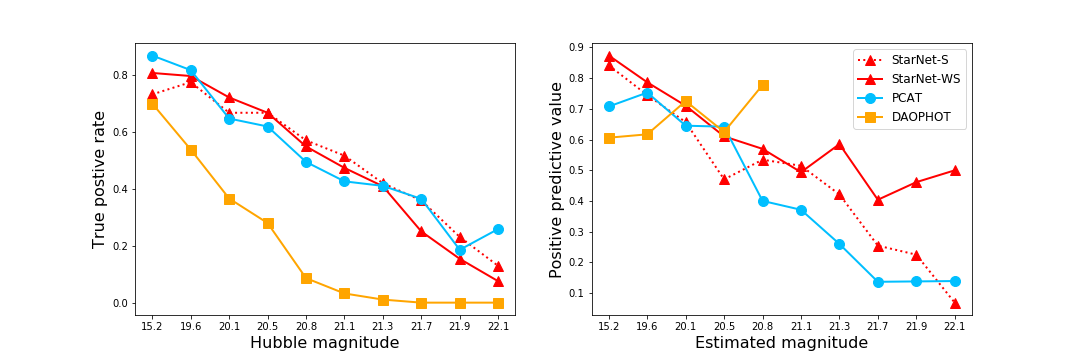
\includegraphics[width=0.99\textwidth]{figures/summary_statistics_m2.png}
    \caption{True positive rate and positive predicted value of various cataloging
    procedures on M2, plotted against magnitude percentile.
    Smaller magnitudes correspond to brighter stars. }
    \label{fig:summary_stats}
\end{figure}

% \begin{table}[!tb]
% \centering
% \caption{Performance metrics on M2.
% For probabilistic methods (StarNet and PCAT)
% the ``\#stars" column refers to the mean number of stars under the (approximate) posterior, while the right-most column displays the 5-th and 95-th percentiles under the posterior. }
% \label{tab:summary_stats}
% \begin{tabular}{l|ccc|cc}
% \toprule
%      Method &   TPR &   PPV &  F1 score &  \#stars & (q-5\%, q-95\%)\\
% \midrule
%     DAOPHOT &  0.20 &  0.63 &      0.30 &     295 & -- \\
%        PCAT &  0.56 &  0.40 &      0.47 &    1672 & (1664, 1680)\\
%  Sleep-only &  0.51 &  0.47 &      0.49 &    1292 & (1260, 1324)\\
%  Wake-sleep &  0.51 &  0.60 &      0.55 &     1014 & (987, 1041)\\
%      %Hubble &  1.00 &  1.00 &      1.00 &     1114 & -- %\\
% \bottomrule
% \end{tabular}
% \end{table}

\begin{table}[!tb]
\centering
\caption{Performance metrics on M2.
For probabilistic methods (StarNet and PCAT)
the ``\#stars" columns provide the mean along with the 5th and 95th percentiles
for the number of stars under the (approximate) posterior,
The number of stars in the Hubble catalog is 1114. }
\label{tab:summary_stats}
\begin{tabular}{l|ccc|cc}
\toprule
& & & & \multicolumn{2}{c}{\#Stars} \\
     Method &   TPR &   PPV &  F1 score &  mean & (q-5\%, q-95\%)\\
\midrule
    DAOPHOT &  0.20 &  0.65 &      0.31 &     357 & -- \\
       PCAT &  0.55 &  0.37 &      0.44 &    1672 & (1664, 1680)\\
 StarNet (our) &  0.53 &  0.48 &      \textbf{0.50} &    1462 & (1430, 1497)\\
\bottomrule
\end{tabular}
\end{table}


\begin{figure}[h]
    \centering
    \vspace{-3cm}
    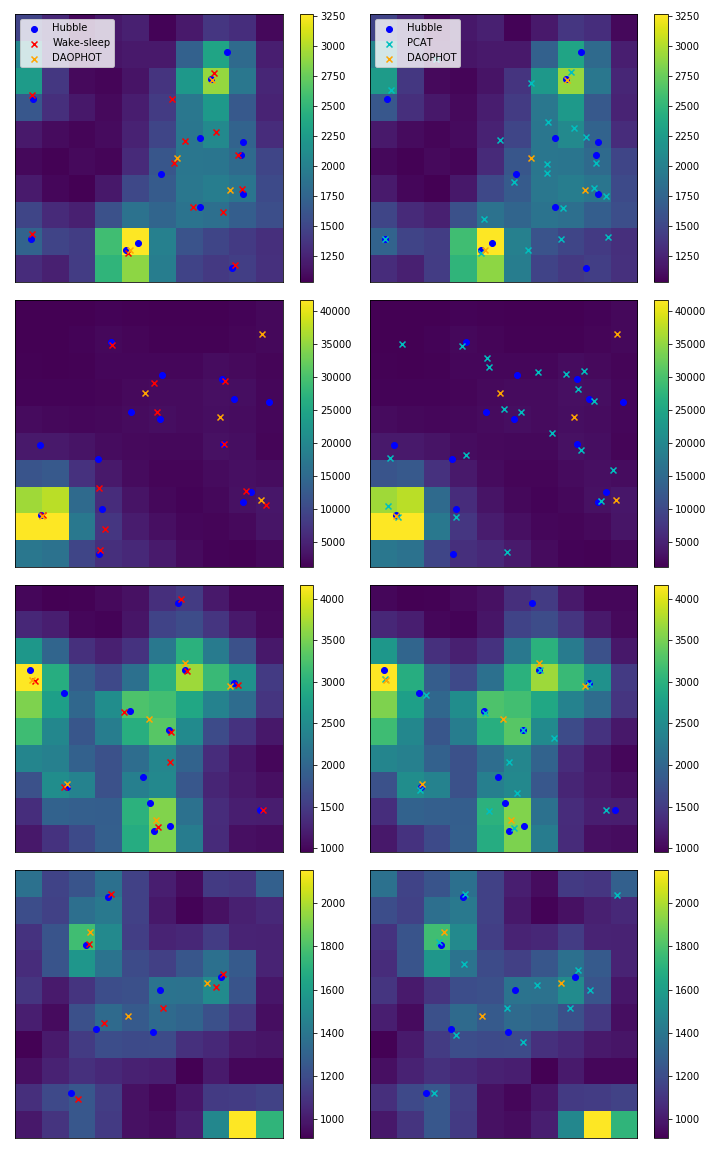
\includegraphics[width=0.8\textwidth]{figures/example_subimages.png}    
    \vspace{-3cm}
    \caption{Estimated catalogs on four 10$\times$10 subimages from 
    M2. Blue dots are Hubble stars brighter than the 22nd magnitude. 
    Starnet, Portillos, and DAOPHOT estimated stars are in 
    red, cyan, and orange x's, respectively. }
    \label{fig:example_subimages}
\end{figure}

\begin{figure}[h]
    \centering
    \vspace{-3cm}
    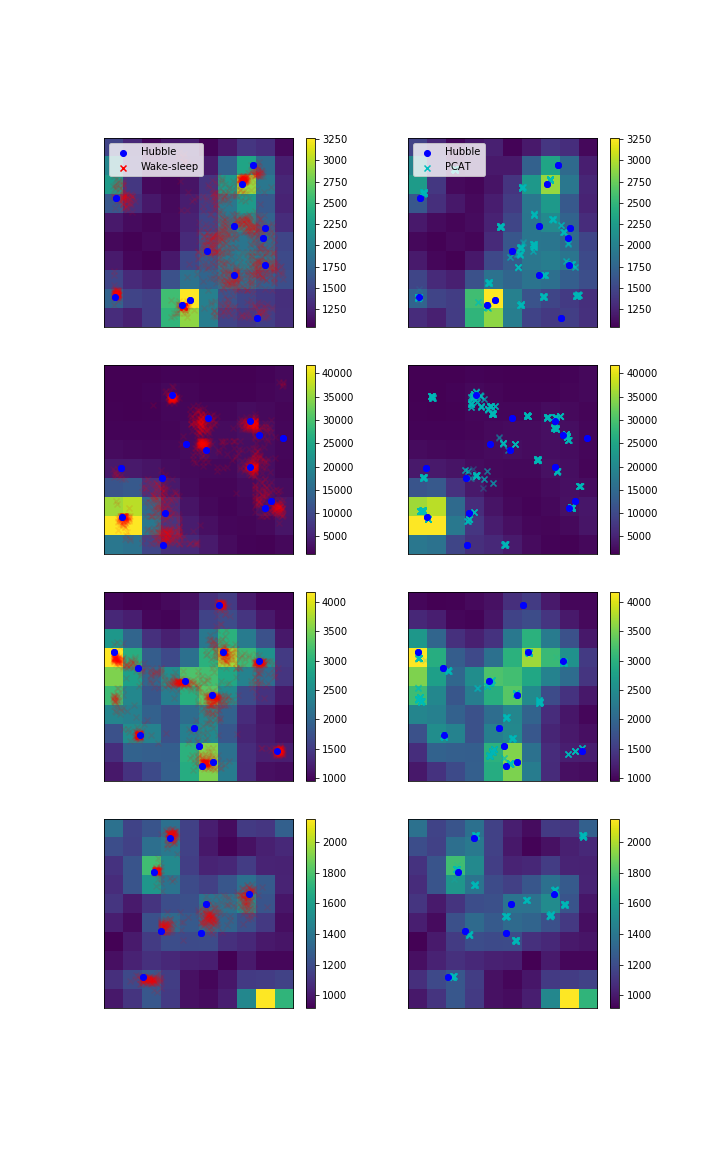
\includegraphics[width=0.8\textwidth]{figures/example_subimages_samples.png}    
    \vspace{-3cm}
    \caption{Four 10$\times$10 subimages from 
    M2. Blue dots are Hubble stars brighter than the 22nd magnitude. 
    We print display the posterior samples from our variational 
    posterior (left) and from the MCMC chain of Portillos (right). }
    \label{fig:example_subimages_sampled}
\end{figure}

\begin{figure}[h]
    \centering
    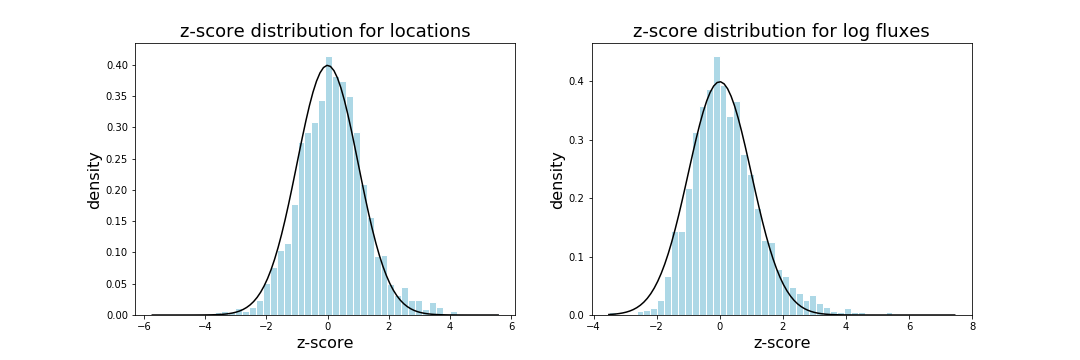
\includegraphics[width=0.99\textwidth]{figures/z-score_calibration.png}    
    \caption{The calibration of uncertainties in our variational posterior. Conditional on the true number of stars, we compute the z-score of the true location or log flux evaluated at our 
    variational posterior. }
    \label{fig:z-score_calibration}
\end{figure}


\begin{figure}[h]
    \centering
    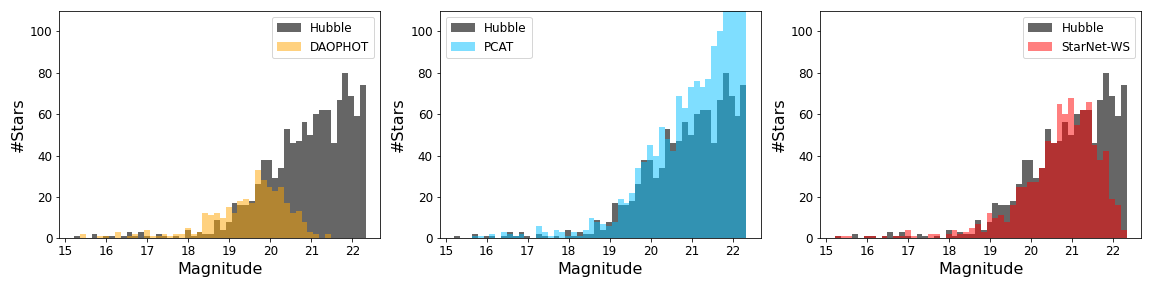
\includegraphics[width=0.99\textwidth]{figures/luminosity_fun.png}
    \caption{Source magnitude histograms on M2. }
    \label{fig:luminosity_fun_m2}
\end{figure}

\begin{figure}[h]
    \centering
    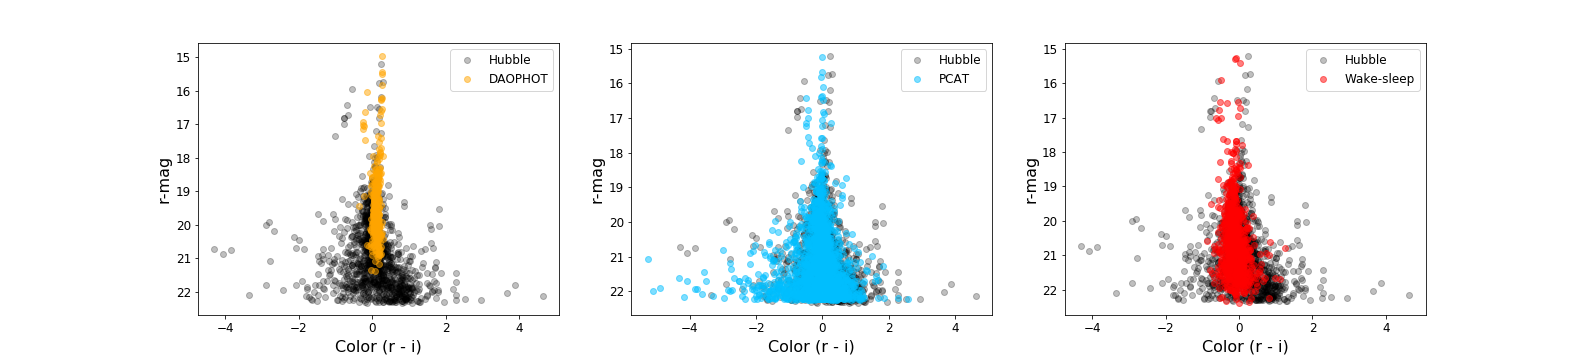
\includegraphics[width=0.99\textwidth]{figures/cmd.png}
    \caption{Color magnitude diagrams on M2. }
    \label{fig:cmd_m2}
\end{figure}


\subsection{Estimation of model parameters}
\input{tables/chi_sq_stats.txt}

\begin{figure}[h]
    \centering
    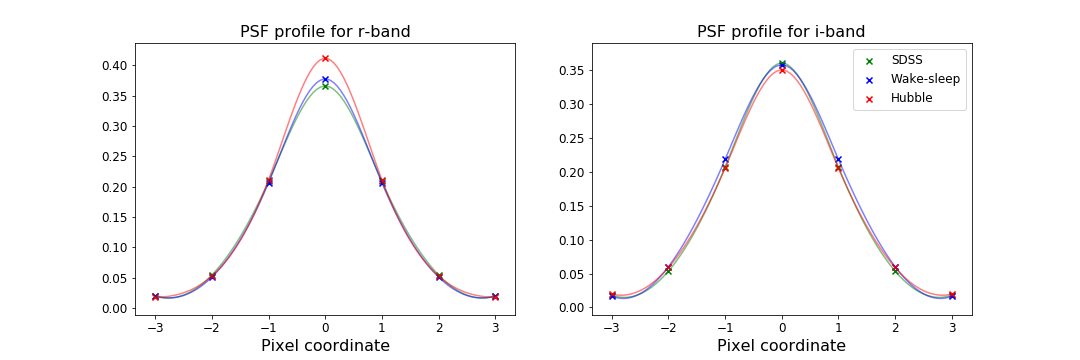
\includegraphics[width=0.99\textwidth]{figures/psf_profiles.png}
    \caption{Estimated versus true PSF profiles on M2. The Hubble PSF was
    obtained by optimizing the likelihood conditioned on locations and fluxes
    from the Hubble catalog. }
    \label{fig:psf_profiles}
\end{figure}


% \multicolumn{1}{p{5cm}}{\raggedleft Chi sq. \\ (with Hubble back.)}
% \caption{
% Chi-squared statistics for SDSS, wake-sleep, and Hubble estimated model parameters.
% The chi-squared statistic is defined as
% $\sum_{bij}\frac{([\text{obs.image}]_{bij} - [\text{recon.image}]_{bij})^2}{[\text{recon.image}]_{bij}}$.
% In the middle column, ``model parameters" refer to both background and PSF.
% In the right column, we fix the background to the Hubble estimate, and examine
% chi-squared statistics as the PSF varies.}



\bibliographystyle{unsrt}
% \bibliographystyle{Chicago} doesn't work
\bibliography{bibliography}
\end{document}
